%!TEX encoding=UTF-8 Unicode

\documentclass[10pt, conference, compsocconf,pdftex,dvipsnames]{IEEEtran}

%=========================encodage fontes et langue=============================

\usepackage[utf8]{inputenc}
\usepackage[english]{babel}
\usepackage[T1]{fontenc}    % (pour les accents)

%===============================================================================

%========================= Todo notes  =========================================


\usepackage{todonotes}
\newcommand{\mytodo}[1]{\todo[inline]{#1}}
%===============================================================================

%========================= gestion des hyperliens ==============================

\usepackage{algpseudocode}
\usepackage{algorithm}
\usepackage{cite}
\usepackage{url}
\usepackage{hyperref}
\hypersetup{
    breaklinks=true, %permet le retour à la ligne dans les liens trop longs
    urlcolor= blue, %couleur des hyperliens
    linkcolor= black, %couleur des liens internes
bookmarksopen=true} 

%===============================================================================

%=========================Mathématiques========================================

\usepackage[cmex10]{amsmath} 
\usepackage{array} % tableaux pour les matrices

\newcolumntype{C}[1]{>{\centering\let\newline\\\arraybackslash\hspace{0pt}}m{#1}}

%===============================================================================

%==========================inclusion d'images===================================

%\usepackage[pdftex]{graphicx} % \includegraphics
\usepackage{caption}
\graphicspath{{./img/}}
\makeatletter
\let\MYcaption\@makecaption
\makeatother
\usepackage[font=footnotesize]{subcaption}

\makeatletter
\let\@makecaption\MYcaption
\makeatother
\usepackage{dblfloatfix}

\usepackage{epstopdf}

%===============================================================================

%==========================listes et mise en page===============================

%\usepackage{paralist} % listes : enumerate, itemize
%\frenchbsetup{StandardLists=true} %pour avoir des listes avec des points

%\usepackage[usenames,dvipsnames]{color} %de la couleur

%\usepackage{appendix} %Annexes

%===============================================================================

%=========================déclaration de titre=================================

\author{\IEEEauthorblockN{David Beniamine, Guillaume Huard}
    \IEEEauthorblockA{
        Université Joseph Fourier\\
        Laboratoire d'Informatique de Grenoble - Inria\\
        38330 Montbonnot St Martin, France\\
    david.beniamine@imag.fr, guillaume.huard@imag.fr}
}

\title{Reducing the impact of communication times on heterogeneous
applications scheduling using KAAPI }

%===============================================================================

\begin{document}

%==========================page de présentation================================


\maketitle%affichage du titre
\begin{abstract}
    \mytodo{Full Rewrite when text is complete}
    High Performance Computing machines use more and more Graphical Processing
    Units as they are very efficient for homogeneous computation such as
    matrix operations. However before using these accelerators, one has to
    transfer data from the processor to them which can be slow. 

    In this study, our aim is to reduce the impact of communication times on
    the makespan of a scheduling. Indeed, with a better anticipation of these
    communications, we could use the GPUs even more efficiently. More
    precisely, we will focus on machines with many GPUs and on applications
    with a low ratio of computations over communications. 

    During this study, we have implemented two offline scheduling algorithms
    within  XKAAPI's runtime.  We have experimentally shown that, by combining
    communication aware scheduling algorithms, we can reduce substantially the
    makespan of a fine grain application.

    Finally our experiments have shown the impact of contention on the PCI bus
    on the makespan of mixed CPU/GPU applications. Moreover we have shown that
    even communications aware scheduling algorithms can be biased when their
    performance model doesn't consider the contention.

\end{abstract}

\begin{IEEEkeywords}
    GPU; Clustering; Scheduling; XKAAPI; Communications;

\end{IEEEkeywords}



%===============================================================================

%=========================début réel du document==============================
\mytodo{Verify all hyperefs}
\section{Introduction}

To obtain portable performances, some runtimes such as XKAAPI
\cite{gautierxkaapi} or StarPU \cite{augonnet2011starpu} allow the programmer
to describe an application such as a set of tasks and dependencies.  They use
a workstealing algorithm \cite{blumofe1995cilk} to schedule theses tasks on
the available resources. As it provide a good load balancing, this algorithm
is quite efficient on homogeneous machines. However nowadays, HPC computers
includes many GPUs, which implies a lot of costly communications. Hence the
basic workstealing algorithm which doesn't manage theses communications can
provide bad performances.

\subsection{List scheduling algorithms}

%%% TODO : explain more the algorithms
The workstealing algorithm is an adaptation of the list scheduling which
provide a makespan $\omega\leq2\omega^*$ where $\omega^*$ is the optimal
makespan \cite{GrahamRL1966Bounds, GrahamRL1969Bounds}. However this bound is
true for homogeneous processors and with no communications. In a model with
heterogenous machines and no communications, this bounds grows to
$\omega\leq\min(s+2-\frac{2s+1}{n},\frac{n+1}{2})\omega^*$ where $s$ is the
number of different resources and $n$ the number of processors. Hence it
doesn't scale for current HPC computers. 

Earliest Task First\cite{hwang1989scheduling} is an adaptation for a finite
number of identical processors with a unitary communication cost between each
couples of processors and without contention. While some tasks aren't
scheduled, the algorithm try to map the earliest task that can be executed on
the processor which minimize it starting time. This algorithm provide a bound
of $\omega\leq(2+c)\omega^*$ where $c$ is the maximum cost of one
communication.  

Heterogeneous Earliest Finish Time \cite{topcuoglu2002performance}  is a two
steps algorithm: first it sort all tasks by non increasing upward rank
(outgoing mean communications and executions time). Then it assign each tasks
to the processor which minimize its finish time. This algorithm is not exactly
a list algorithm as it allow a processor to remain idle while a task is ready
to be executed.  Hence it doesn't provide any bound on the execution time
moreover recent work have shown that the worst case can provide a makespan
$\omega \geq \frac{m}{2}\omega^*$ where $m$ is the number of tasks
\cite{Kedad-SidhoumMonnaMounieEtAl2013}. Despite this results, the HEFT
algorithm is widely used (by StarPU and XKAAPI amongst others), and give some
good results in many case\cite{ferreiralima:hal-00735470}. Nevertheless, the
same study have shown that in some case this algorithm give better results
when we use only the half of the available GPUs.

If most of these algorithms are designed offline, they are often implemented
online on the runtimes scheduler. These online adaptations have a lower cost
than the original, however the neglect the outgoing work of a task when they
compute its schedule. Therefore the offline version should be more efficient
when the communications are costly.

\subsection{Clustering Algorithms}

Clustering algorithms are designed for an unbounded number of processors, they
consider the structure of the DAG and group tasks into clusters. All the
tasks which belong to one cluster are assigned to the same processor (i.e. 
there are no communication between them).  

One of the most known clustering heuristic is the Dominant Sequence
Clustering\cite{yang1994dsc}, it assigns to each task a priority corresponding
to the sum of the longest path from a root node to this task and the longest
path from this task to a sink node.Then the algorithm sort the tasks by
decreasing priority and try to affect each task to the cluster which minimize
its start time among the cluster containing its predecessors. However if a
task can start earlier when we assign it to a new cluster instead of assigning
it to an existing one, we create a new cluster for this task.

The idea of CLANS
\cite{aubum1990efficient,mccreary1993partitioning,mccreary1993graph} is to
decompose the DAG into a tree of clans representing a recursive expression of
the relationship between tasks. For a graph $G=(V,E)$, a set of nodes
$X\subset V$ is a clan of the graph $G$ if and only if $\forall (x,y) \in X,
\forall z \in V-X$, $z$ is an ancestor (or successor) of $x$ if and only if
$z$ an ancestor (resp. successor) of $y$. There are three types of clans:
Independent, linear and primitive. Once the graph is decomposed into clans,
the algorithm traverse the tree bottom up using the communication and
execution times to determine if two clans have to be merged or not.

\begin{figure}[htb]
    \centering
    \includegraphics[width=0.33\textwidth]{conv.png}
    \caption{Convex and non convex group of tasks.}
    \label{fig:conv}
\end{figure}


The convex clustering algorithm\cite{lepere2002new} produces an acyclic graph
of clusters.  Indeed a cluster $C$ is convex if and only if $\forall\ (x,z)\
\in\ C$ all task $y$, such that $x\ \prec\ y\ \prec\ z$, is in $C$ (see
figure \ref{fig:conv}). By this property, we know that there are no two way
communications between two clusters. Moreover as the graph obtained by merging
the tasks inside a cluster is a Direct Acyclic Graph, it allow us to run
any scheduling algorithm on it.

A theoretical comparison\cite{khan1994comparison} between the algorithms DSC,
MCP (Modified Critical Path, similar to DSC), MH, HU (lists algorithms) and
CLANS have shown that CLANS is robust and efficient for a large and diverse
set of graphs. All the others algorithms give very bad performances for graphs
with a low ratio computation over communications (also called grain). 

\subsection{Key Issues}

Although the GPUs are able to reduce substantially the execution time of
some tasks, we need to transfer data from the main memory to them before
the execution. Previous work\cite{ferreiralima:hal-00735470} have shown
that it is possible to reduce the impact these communications costs by
overlapping them with computation and by using sophisticated scheduling
algorithms such as HEFT.  However, this work have also highlighted the
fact that some contention can occur on machine with many GPUs linked to
the processors by an interconnection network.

In this study, we will use machines with one or several GPUs, aiming to
show and to measure the impact of the communication times on the
scheduling of HPC applications. As all the list scheduling algorithms cited
before are efficient for coast grain applications, we have focused our
analysis on very fine grain applications. 

To reach that goal, we have implemented a static scheduler and several
heuristics within the parallel runtime XKAAPI. We have combined list
scheduling algorithms and clustering heuristics to reduce the impact of
communications. Using our scheduler, we have led an experimental study
showing that the offline version of HEFT can give a gain of $59\%$
compared to the makespan of the online one when the volume of
communications is large enough. Moreover, using a clustering algorithm
before HEFT, we have reduced the makespan of one scheduling up to $64\%$
compared to the online HEFT.

First we will present our implementation of the convex cluster algorithm in
XKAAPI's runtime, and the adaptation that we have made in section
\ref{sec:impl}. Then we will use this scheduler to analyse the impact of
communication in section \ref{sec:exp}. And finally we will give our
conclusion and some future work on section \ref{sec:cncl}.

\section{Implementation of an offline scheduler in XKAAPI's runtime}
\label{sec:impl}

By default, XKAAPI uses an online scheduler and compute data dependencies in a
lazy way, nevertheless to study the impact of communications and to run
structural algorithms, we have decided to work with an offline scheduler.
Still the online heuristic work with actual time when the offline one uses
predicted times thus only the first one is able to adapt to unexpected effects
such as contention. XKAAPI's scheduler provides various heuristics, among
them, we can find an online adaptation of the HEFT algorithm. The main
difference between this online version and the original one is that the first
one cannot sort the ready tasks as the DAG is not fully known.

At first, we have compared the online adaptation of the HEFT algorithm with an
offline version, using linear algebra applications, as this heuristic do not
consider the communication times as much as the original one.  Then we have
tried the static scheduler with and without a clustering phase before the HEFT
algorithm to take even more the communications into account. 

\subsection{XKAAPI scheduler and performance model}
\label{sec:impl-kaapi}

XKAAPI has an API for writing scheduling heuristics, however as it is designed
for online algorithms this interface is quite limited. We can basically write
three callbacks methods, the first is launched during the initialization of
the runtime before the execution of the program. The second one is called each
time a tasks is ready to be executed and must return the processor on which
the tasks should be run. The last one is called when a processor wants to
steal a task from another and must return the task to be stolen.

Although this API is minimalistic, as we can extract the DAG from the ready
tasks list during the initialization, we are able to run an offline scheduler
during this phase and apply its decision when the runtime calls the
\texttt{push} and \texttt{steal} functions. However this interface do not
enable us to force the order of execution of two tasks. Thus we need to add
some (empty) internal tasks to enforce dependencies between tasks which belong
to different clusters.

XKAAPI have also a performance model which provide for each task a prediction
of its execution time on a each processor. This model can also estimate the 
time needed to transfer $n$ bytes of data from one processor to an other. This
predictions are made from the traces of one (or many) previous calibration
runs. We will discuss the impact of these previous runs an how this model can
be biased in section \ref{sec:exp}. It is important to notice that even the
online adaptation of HEFT uses this performance model.

\subsection{Offline scheduling}
\label{sec:impl-off}
By default, in XKAAPI, each processor has a part of the work in his queue of
tasks, nevertheless the XKAAPI's C++ API allow to spawn tasks with the keyword
\texttt{SetStaticSched} which force XKAAPI to maintain a centralized list of
ready tasks. As each task has a pointer to all its successors, the
dependencies graph is known within the runtime. However as the convex cluster
algorithm require a test of the relationship between almost every pairs of
vertices of the DAG,  with this pointer based representation, computing these
relationships can be costly. Therefore the first step of our static scheduler
is to extract the DAG into an adjacency matrix and to run a Warshall Algorithm
which compute all the parenthood relations. Although this algorithm have a
worst case in $O(|V|^3)$ for a graph $G=(V,E)$, and a mean case in $O(|V|^2)$
it is worthwhile as it allow us to know in constant time if two nodes are
related or not.

Once these dependencies are computed, we are able to run our implementation of
the convex cluster algorithm (see algorithm \ref{algo:conv-clust}). The
original convex cluster algorithm select two independent random nodes and use
them to divide the group into four partitions $A$ and $A^{\sim}$ which are
independent, their predecessors $A^<$ and successors $A^>$. Once these
partitions are computed, either the smallest of $A$ and $A^{\sim}$ is large
enough and all the partition are recursively divided, or they are all grouped
into one cluster. 

Our implementation is close to this algorithm however as it is designed for a
theoretical machine with an unbounded number of identical processors, it
requires a few adjustments, for example in the original version the recursion
stops when the partition size is less than twice the communication cost. As we
do not have a unitary communication cost, we have decided to fix a maximal
size for a cluster and to stop the recursion when a cluster is smaller than
this size (see line \ref{algop:rec-stop}). Then, the clusters are mapped on the
processors using the HEFT algorithm. 

\begin{algorithm}[htb]
    \centering
    \caption{Convex cluster}
    \label{algo:conv-clust}
    \begin{algorithmic}[1]
        \Function{Extract\_clusters}{Graph $G=(V,E)$}
        \State $Part \gets NULL$
        \State $CurMax \gets 0$
        \For{$rdt \in  [0 .. MaxRandomTry ]$ }\label{algop:main-loop}
        \State $pivot \gets RandomNode(G)$
        \State
        $<A,A^{\sim},A^<,A^>>=Decompose\_4\_parts(G,pivot)$\\\label{algop:init-part}
        \Comment Decompose G into four partitions $pivot$, nodes independent from $pivot$,\\ 
        \Comment $pivot$'s ancestors and $pivot$'s successors\\
        \Comment see figure \ref{fig:conv-decomp1}, \textbf{Cost: $O(|V|)$}
        \State $Update\_partitions(<A,A^{\sim},A^<,A^>>)$
        \\\label{algop:update-part}
        \Comment $A^<$ and $A^>$ becomes predecessors  (respectively successors)\\
        \Comment of all nodes from $A$ and $A^{\sim}$, see figure \ref{fig:conv-decomp2} \\
        \Comment \textbf{Cost:$(|A^<| +
        |A^>| )*|A^{\sim}| = O(|V|^2)$}
        \If{$MAX(|A|,|A^{\sim}|) > CurMax$} \label{algop:part-choice}
        \Comment We have found a better decomposition
        \State $CurMax \gets MAX(|A|,|A^{\sim}|)$
        \State $Part \gets <A,A^{\sim},A^<,A^>>$
        \EndIf
        \EndFor
        \ForAll{$p \in Part$}
        \If{$|p| > MaxClusterSize$}\label{algop:rec-stop}
        \State $Extract\_Clusters(p)$
        \Comment Divide the partition if big enough
        \Else
        \State $Add\_Cluster(p)$
        \Comment Save the cluster
        \EndIf
        \EndFor
        \EndFunction
    \end{algorithmic}
\end{algorithm}

\begin{figure*}[tb]
    \centering
    \begin{subfigure}{0.24\textwidth}
        \centering
        \includegraphics[width=0.7\textwidth]{conv-decomp0.png}
        \caption{Original graph.}
        \label{fig:conv-decomp0}
    \end{subfigure}
    ~
    \begin{subfigure}{0.27\textwidth}
        \centering
        \includegraphics[width=0.7\textwidth]{conv-decomp.png}
        \caption{\texttt{Decompose\_4\_parts()}}
        \label{fig:conv-decomp1}
    \end{subfigure}
    ~
    \begin{subfigure}{0.27\textwidth}
        \centering
        \includegraphics[width=0.7\textwidth]{conv-decomp2.png}
        \caption{\texttt{Update\_Partitions()}}
        \label{fig:conv-decomp2}
    \end{subfigure}
    \caption{Decomposition and update step of convex cluster algorithm.}
    \label{fig:conv-decomp}
\end{figure*}


In addition, some experiments showed that the original criterion used to
determine which clustering was the best among the random test gave unstable
performances. Hence we have decided to change it to keep always the clustering
giving the largest cluster (see line \ref{algop:part-choice}), and we have
shown that this heuristic gave better results. Finally, we choose to
recursively divide each individual clusters if it is large enough (line
\ref{algop:rec-stop}) while the original algorithm divide either all the
clusters or none of them.

The two important (and costly) steps of this algorithm are the initial
decomposition into four clusters, and their update to keep the clusters
balanced.  Starting from the graph shown on figure \ref{fig:conv-decomp0}, we
choose randomly a pivot (the node $7$) and we put all the others nodes in one
of the three groups its predecessors $A^<$, its successors $A^>$ all the
others $A^{\sim}$. At the end of this step we have the clustering displayed on
figure \ref{fig:conv-decomp1}. As we can know in $O(1)$ the relationship
between two nodes, this step costs only $O(|V|)$ comparisons. During the second
step, we compare each nodes of $A^<$ and $A^>$ with the nodes of $A^{\sim}$ to
determine the common predecessor (resp successors) of $A$ and $A^{\sim}$ keep
their initial placement, the others are moved in the group $A$.  By this way
we obtain the clustering presented on figure \ref{fig:conv-decomp2}. The
second step has a cost of:
$$C=(|A^>|+|A^<|)*|A^{\sim}|$$ 
we know that at the end of the first step $|A|=1$ which implies: 
$$|A^>|+|A^<|+|A^{\sim}|=|V|-1$$
thus:
$$C=(|V|-1-|A^{\sim}|)*|A^{\sim}|$$ 
The two terms are bounded by $|V|$ so we have: 
$$C\leq|V|^2$$
and so if $|A^{\sim}|=\frac{|V|}{2}$,
$$C=(|V|-1-\frac{|V|}{2})*\frac{|V|}{2}=\left(\frac{|V|}{2}\right)^2-\frac{|V|}{2}$$
hence we have: 
$$C=O(|V^2|)$$ 
Finally, if we assume that the clusters are balanced it takes
$log\left(\frac{|V|}{MaxClusterSize}\right)$ calls to stop the recursion, as
the two first step are repeated $MaxRandomTry$ times, the
cost of our implementation is:
$$O\left(MaxRandomTry*|V|^2*log\left(\frac{|V|}{MaxClusterSize}\right)\right)$$

As the clustering phase aim of increasing the grain of the graph, we need to
be sure that each cluster will behave as one big task. Therefore in the
runtime, we have to add some empty synchronization tasks at the beginning and
at the end of each clusters as shown in figure \ref{fig:conv-int} (white
diamond shaped nodes). Indeed with the clusters of the figure
\ref{fig:conv-decomp2}, without these tasks,  as XKAAPI use a work stealing
algorithm to execute a tasks as soon as it is ready, if the clusters $A^<$ and
$A^{\sim}$ are executed on the same processor, the second one might start
before the end of the first, delaying the execution of the cluster $A$.
Although these synchronization tasks increase the size of the graph, they are
empty, and as the cost of a tasks is very low in XKAAPI, the overhead induced
by is negligible. Once the DAG of clusters has been computed, we can find the
mapping between the clusters and the processors according to the HEFT
algorithm for instance. 

\begin{figure}
    \centering
    \begin{subfigure}{0.24\textwidth}
        \centering
        \includegraphics[width=0.7\textwidth]{conv-internal.png}
        \caption{Graph after adding the internal tasks.}
        \label{fig:conv-int}
    \end{subfigure}
    ~
    \begin{subfigure}{0.1\textwidth}
        \centering
        \includegraphics[width=\textwidth]{conv-clust.png}
        \caption{Cluster graph.}
        \label{fig:conv-clust}
    \end{subfigure}
    \caption{Final transformations from a graph of tasks to a graph of
    clusters.}
    \label{fig:conv-end}
\end{figure}



This two step have a cost $\leq |V^2|$ hence our offline scheduler has a
theoretical worst case cost in $O(|V|^3)$ due to the Warshall algorithm,
however the mean case cost is still $O(log(|V|)*|V|^2*MaxRandomTry)$ (due to
the convex cluster algorithm).  Although this cost is quite high, in some
domains such as physical simulation or signal analysis, applications are often
iterative and regular. This means that the same parallel code has the
opportunity to be executed several times in a row using the same schedule.
Hence we can amortize that initial cost. As our aim is to study the impact of
communication times, we will not try to amortize this initial cost in the
following experiments and we will separate it from the execution times in our
results.

\section{Analysis and reduction of the communication times}
\label{sec:exp}
Using our scheduler, we have studied the impact off communications on two
different machines which are described in section \ref{sec:exp-set}. For this
experimental analysis we have compared the online HEFT with our offline
implementation and we have combined it with a clustering phase.

\subsection{Experimental setup}
\label{sec:exp-set}

\begin{table*}
    \centering
    \scalebox{0.78}
    {
        \begin{tabular}{|C{1.7cm}|c|C{1.1cm}|C{1.3cm}|C{1.2cm}|C{1.2cm}|C{1.6cm}|
            C{1.3cm}|C{1.4cm}|C{1.2cm}|C{1.6cm}|C{1.4cm}|C{1.8cm}|}
            \hline
            \textbf{Name} & \textbf{\#CPU} & \textbf{\#Core / CPU} 
            &\textbf{ CPU vendor} & \textbf{CPU model}  &
            \textbf{CPU freq (Ghz)} & 
            \textbf{Memory (Gio)} & \textbf{\#GPU} & 
            \textbf{GPU vendor} & \textbf{GPU model} &  
            \textbf{GPU memory}&\textbf{GPU clock freq (Ghz)} 
            &\textbf{ CUDA capability} \\
            \hline
            Mapuche & 1 & 4 & Intel & Core I7-2600 & 3.4 & 8 & 1 & Nvidia &
            NVS 300 & 512 MB DDR3& 1.23 &1.2 \\
            \hline
            IdGraf & 2 & 6 & Intel & Xeon X5650 & 2.67 & 72& 8 & Nvidia &
            Tesla C2050 & 3GB GDDR5 & 1.15 & 2.0 \\
            \hline
        \end{tabular}
    }
    \caption{Hardware used for the experiments.}
    \label{table:machines}
\end{table*}

All the experiment presented in this study, have been run on one or the other
of the two following machines:
Idgraf\footnote{\url{http://digitalis.inria.fr/index.php/Usage\#idgraf}} a HPC
workstation with 12 cores and 8 GPUs managed by Grid5000 and Mapuche a
personal workstation with 4 CPUs and one GPU. The hardware of these machines
is described more precisely in table \ref{table:machines}, for both machines
we hyper-threading and thermal throttling are turned off. 

Idgraf runs on a Debian squeeze with a Linux kernel
3.2.0.2-amd64. Mapuche's Operating System is an Ubuntu 12.10 LTS with a
Linux kernel 3.2.0-40. 


\begin{figure}[htb]
    \centering
    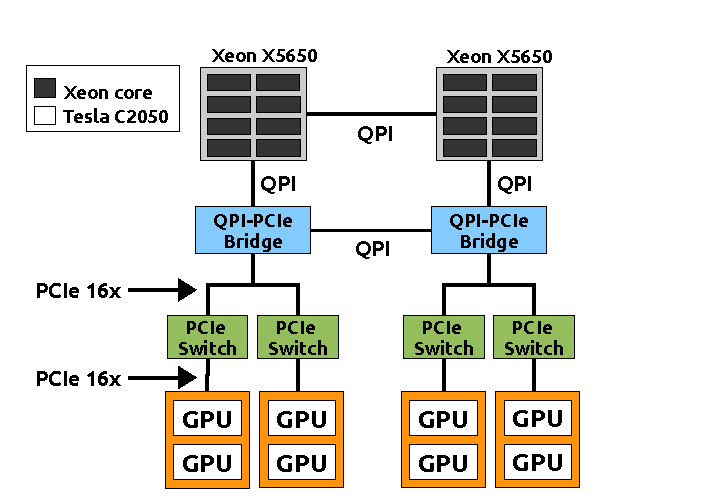
\includegraphics[width=0.48\textwidth]{idgraf-topo-2012.pdf}
    \caption{Idgraf's topology\cite{gautierxkaapi}.}
    \label{fig:idgraf}
\end{figure}

It is important to note that Idgraf has a hierarchical topology as shown in
figure \ref{fig:idgraf}, the eight GPUS are split over two PCI Bridge which
are linked together. Each bridge manage 4 GPUs separated in two groups which
belong to two different switches. With this particular topology, simultaneous
communications involving several GPUs might led to contention on the PCie switches,
this contention will be highlighted in section \ref{sec:exp-exp-perf}.

Concerning our algorithms, unless stated otherwise, we use the following
parameters:\\
$NbRandomTries=\sqrt{|V|}$, $MaxClusterSize=10$, and for the
studied applications\\
$MatrixSize=1000$, $BlocSize=MatrixSize/10$.

For each curve presented in the following sections, each points represent the
mean runtime of at least 15 different runs with the same parameters, and a
confidence interval of $95\%$ is displayed as an error bar.

Finally, by default the execution time presented for the algorithms HEFT
offline, and convex cluster correspond to the total time minus the overhead
induced by the static scheduler.


\subsection{Comparison of online and offline heuristics}
\label{sec:exp-exp-perf}

There are two important differences between the online and the offline version
of the HEFT algorithm, the first one is that the offline algorithm sorts the tasks
by upward rank, which mean that a task priority is related to the length of
the chain of tasks that depends on it. As the online version does not have a
global vision of the DAG, it maps tasks to processors as soon as they are
ready, without sorting them which can result on bad scheduling choice. However
the second difference is that the offline algorithm only uses theoretical
execution and communication times while the online one uses theoretical times
for predictions but makes it decision at the runtime. Hence if there is some
contention, the online algorithm will see that a processor which should be
ready isn't and will adapt it's decisions.

To show these differences, we have compared the makespan of a Cholesky
reduction on our two machines using all the available GPUs  with the two
versions of HEFT. The results are displayed in figure \ref{fig:OnOff}. The
first important point is that, on Mapuche (figure \ref{fig:OnOffMapuche}), the
offline algorithm provide always an equivalent or better makespan than the
online one. In the best case we have observed a gain of $59\%$. This
result confirms our first idea when we are in a configuration where there are many
communications and not enough computations to overlap them, we can
obtain a substantial gain by using an heuristic aware
of these communications. 
\begin{figure}[htb]
        \addtocounter{figure}{1}
        \centering
        \begin{subfigure}{0.5\textwidth}
        \scalebox{0.6}{
            \input{img/gpu-idgraf-c0-cal1GPU-off.tex}
        }
        \caption{Effect of the number of GPUs used during the execution.}
        \label{fig:ContentionGpu}
    \end{subfigure}
    \begin{subfigure}{0.5\textwidth}
        \scalebox{0.6}{
            \centering
            \input{img/mat-size-idgraf-8gpu-cal1-8GPU.tex}
        }
        \caption{Effects of the number of GPUs during the calibration.}
        \label{fig:ContentionTrick}
    \end{subfigure}
    \label{fig:Contention}
    \caption{Analysis of the contention, on the execution time of a 
    Cholesky reduction, on Idgraf.}

\end{figure}

\begin{figure*}[bt]
    \addtocounter{figure}{-2}
    %\begin{adjustwidth}{}{-3cm}
    \centering
    \begin{subfigure}{0.4\textwidth}
        \hspace{-20pt}
        \scalebox{0.7}{
            \input{img/mat-size-mapuche-noInt-calibrate.tex}
        }
        \caption{Comparison on Mapuche.}
        \label{fig:OnOffMapuche}
    \end{subfigure}
    \hspace{15pt}
    \begin{subfigure}{0.55\textwidth}
        \scalebox{0.7}{
            \input{img/mat-size-idgraf-8gpu-cal8GPU.tex}
        }
        \caption{Comparison on Idgraf.}
        \label{fig:OnOffIdgraf}
    \end{subfigure}
    %\end{adjustwidth}
    \caption{Online vs offline HEFT scheduling, on Cholesky reduction, on both
    machines.}
    \label{fig:OnOff}
\end{figure*}
\addtocounter{figure}{1}


Nevertheless, the same experiment on Idgraf gives a different result, indeed
we can see in figure \ref{fig:OnOffIdgraf} that if we still have a gain of
$17.7\%$ with a matrix of size $800$. However, when we increase this size, the
gap shrinks and finally, when it exceed $1400$ the online algorithm gives
better results up to $10.2\%$. As the main difference between the two machines
is the number of GPUs and as the advantage of the online scheduler compared to
the offline one is the capacity to adapt to a biased model, our first
hypothesis, is that a contention which cannot be anticipated by the model
appears on the PCI buses (see figure \ref{fig:idgraf}) when we use all the
GPUs. 

To prove this hypothesis, we have run the same experiment on one, two, four
and eight GPUs with both algorithms. The figure \ref{fig:ContentionGpu} shows the
results off the offline heuristic with one and eight GPUs. We can see that we
obtain equivalent or better makespan using only one GPU. We obtain the same
results with the online algorithm.
%
%Furthermore, if the offline algorithm give better results with only one GPU
%(see figure \ref{fig:Contention1}), with eight we have the opposite result
%(see figure \ref{fig:Contention8}).

In addition, we have found that for many tasks, the predicted execution times
(i.e. the execution time extracted from the calibration runs) were increasing
as we were using more GPUs. As the eight GPUs are identical, this rise means
that our performances model include some communications in the execution times
and these communications takes more time when we use all the available GPUs.
Moreover as this contention appears in our execution times, our algorithms
were biased. However, we can easily avoid this bias by performing our
calibration run with only one GPU. Doing this, we are able to reduce the
execution time of $24.7\%$ on 8 GPUs as we can see on figure
\ref{fig:ContentionTrick}. All these results validate our hypothesis, there is
some contention on the PCI buses.

Finally, we have clearly shown that the offline algorithm is able to give
better results (up to $59\%$ in our experiments) by avoiding some
communications. However, if the model does not fit to the reality (for example
when there is some contention), an online algorithm is more adaptated. Hence
we can think about implementing an hybrid scheduler which takes initial
decisions statically and adapts (or recompute them) if the actual execution
times does not match to the expected ones.

\subsection{Analysis of the clustering algorithm}
\label{sec:exp-exp-clust}

In the following experiments, we have increased the grain of the DAG using the
convex cluster algorithm before running the offline HEFT algorithm. Using this
combination, we will show that we can have even a better gain than with the
offline or the online algorithm only.

\mytodo{refaire la courbe \ref{fig:MatIdgraf}}
\begin{figure*}[tb]
    %\begin{adjustwidth}{}{-3cm}
        \centering
        \begin{subfigure}{0.4\textwidth}
            \hspace{-20pt}
            \scalebox{0.7}{
                \input{img/mat-size-c10-mapuche.tex}
            }
            \caption{Mapuche.}
            \label{fig:MatMapuche}
        \end{subfigure}
        \hspace{15pt}
        \begin{subfigure}{0.55\textwidth}
            \scalebox{0.7}{
                \input{img/mat-size-bm20-m600_1100-4GPU-cal1GPU-idgraf.tex}
            }
            \caption{Idgraf, $BlocSize=MatrixSize/20$.}
            \label{fig:MatIdgraf}
        \end{subfigure}
    %\end{adjustwidth}

    \caption{Square matrix dimension impact on convex cluster and HEFT
    algorithm, on a Cholesky reduction, on both machines.}
    \label{fig:Mat}
\end{figure*}

Our first experiment on the convex cluster algorithm aim at showing for which
matrix size this heuristic can be useful. We can see in figure
\ref{fig:MatMapuche} that as for the offline HEFT, the convex cluster
algorithm give better results for small matrices, with a gain up to $28.5\%$
on Mapuche with a matrix size of $800*800$. Nevertheless, there is still one
parameter of the convex cluster algorithm that we have not tested yet which is
the maximum cluster size. Following experiments will show that with an
appropriate size of cluster, we can get a even better makespan.

On idgraf, to obtain a better scheduling, we had to increase the volume of
communications by decreasing the bloc size. With this parameter, the convex
clustering give a better schedule than the online HEFT as we can see in fiugre
\ref{fig:MatIdgraf}.  The best case tested in our experiment is for a matrix
size of $600*600$ where we reduce the makespan of $64\%$.

From this experiment, it is clear that with small matrices, we can highly
improve the scheduling obtained by the online algorithm. For the next
experiments, we will use a small matrix $1000*1000$ and we will keep the same
bloc sizes as for this experiments. Finally, we are going to study the impact
of the maximal size of one cluster on the scheduling.

\begin{figure*}[tb]
    %\begin{adjustwidth}{}{-3cm}
    \centering
    \begin{subfigure}{0.4\textwidth}
        \hspace{-20pt}
        \scalebox{0.7}{
            \input{img/clust-size-c0-80_m1000_b100-improved-log.tex}
        }
        \caption{Mapuche.}
        \label{fig:ClustersMapuche}
    \end{subfigure}
    \hspace{15pt}
    \begin{subfigure}{0.55\textwidth}
        \scalebox{0.7}{
            \input{img/clust-size-full-bm20-m1000-4GPU-cal1GPU-idgraf.tex}
        }
        \caption{Idgraf, $BlocSize=MatrixSize/20$, $4$GPUs.}
        \label{fig:ClustersIdgraf}
    \end{subfigure}
    %\end{adjustwidth}

    \caption{Effect of the maximum size of clusters on the convex cluster
    algorithm, on a Cholesky reduction, on both machines.}
    \label{fig:Clusters}
\end{figure*}

By increasing the maximum size of a cluster (see algorithm
page \pageref{algo:conv-clust}, \ref{algo:conv-clust}, line
\ref{algop:rec-stop}), we increase the grain of the graph and we reduce the
amount of communications that HEFT has to manage.

Figure \ref{fig:ClustersMapuche} show the results of our last experiment on
Mapuche, we can see that we need large clusters $\geq 30$ to obtain the maximal
gain. However if we use a cluster size larger than $70$, it seems that we
loose to much informations and the HEFT algorithm cannot give an efficient
scheduling anymore. Finally, we can notice that with $MaxClusterSize=35$ we
reduce the execution time by $48.7\%$ in comparison to the online HEFT
algorithm.

In figure \ref{fig:ClustersIdgraf}, we displayed the results of the
experiment on Idgraf using $4$ GPUs, we can see that the best cluster size is
quite different than for Mapuche. This difference comes from the fact that as
Idgraf embed more processors than Mapuche, hence it needs a larger graph (i.e.
smaller clusters) to use them efficiently. Still, with the convex clustering,
we can obtain a gain of $32.3\%$ on Idgraf compared to the online one, while
the offline algorithm only gave a gain of $11.4\%$ (fig
\ref{fig:ClustersIdgraf}, $MaxClusterSize=0$).



\section{Conclusions and future work}
\mytodo{Conclude}
\label{sec:cncl}
+ Complex heuristic helps, but need a good perfmodel, and cost a lot
\\
=> reuse a scheduling 
\\
=> Combine offline init sched + online if too far from predictions
\\
=> More work on perfmodel
\\
+ Different Apps
%===============================================================================

%=========================Bibliographie========================================
%\IEEEtriggeratref{3}

\bibliographystyle{IEEEtran}
\bibliography{ConvexGpu}

%===============================================================================

%=========================annexes==============================================

%newpage
%\appendix{ \textbf{Annexe }}

%===============================================================================
\mytodo{Remove the todo list}
\listoftodos
\end{document}

